\documentclass{article}
\usepackage[utf8]{inputenc}
\usepackage{amssymb,
  amsmath,hyperref,verbatim,listings,graphicx,subfigure,fullpage, braket}
\renewcommand\vec[1]{\ensuremath{\mathbf{#1}}}

\begin{document}

\title{UML computer project 2}
\author{
Juha-Antti Isojärvi\\
013455341 \\
Department of Mathematics and Statistics\\
Master student
\and
Mikko Sysikaski\\
013573016\\
Department of Computer Science\\
Master student}
\date{}
\maketitle

\section{Exercise set 1}
\subsection{Exercise 1}
\begin{figure}\centering
	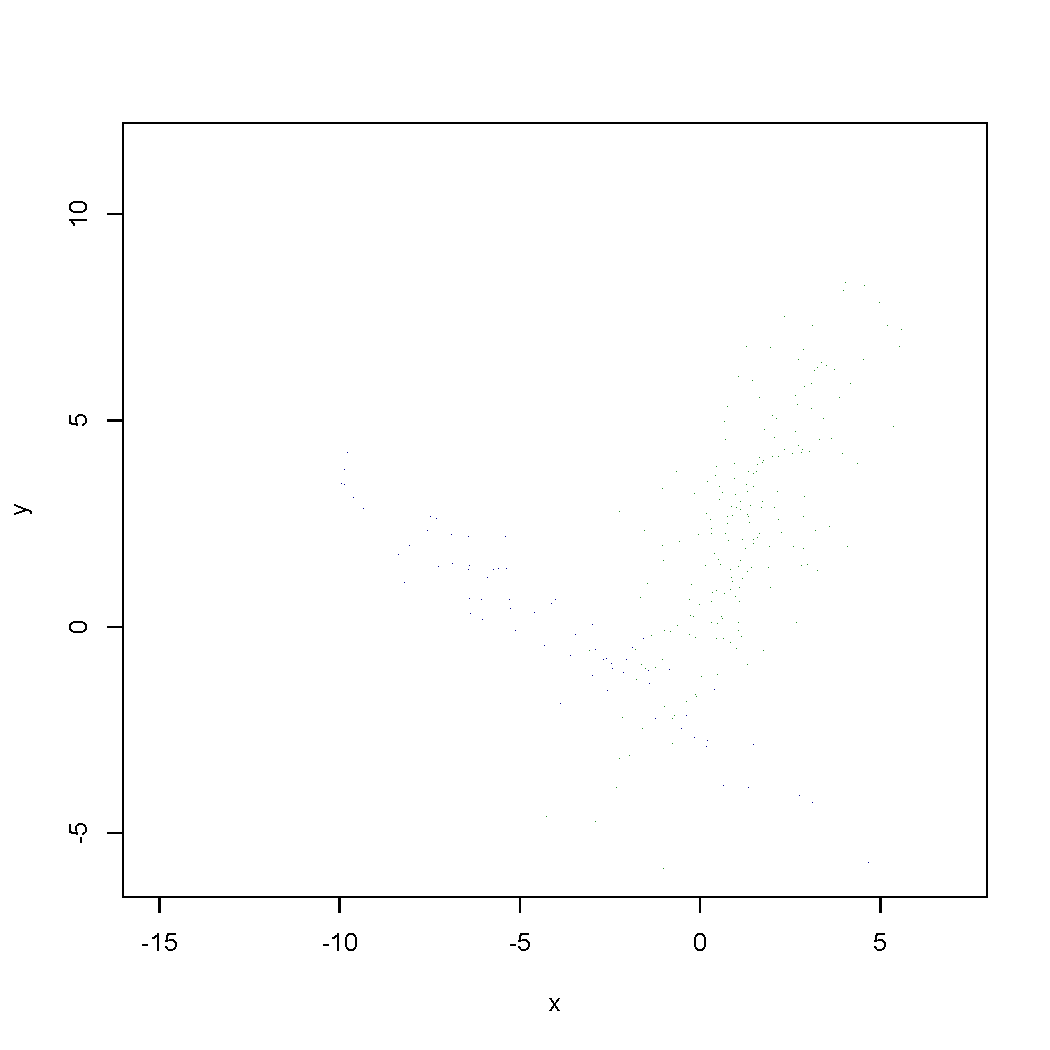
\includegraphics[totalheight=0.5\textheight]{scatterE31.pdf}
	\caption{Scatter plot of the data.} \label{fig:scatterE31}
\end{figure}

\section{Exercise set 2}
\subsection{Exercise 1}\label{sec:ex21}
Multi-dimensional scaling is a projection method that is based on analyzing the distances between the data vectors.
Let $\vec X=(\vec x_1,\dots,\vec x_N)$ be the data matrix to be analyzed.
Each $\vec x_i$ is a column vector of length $n$.
In linear MDS we look at the distance matrix where the elements are defined by $d_{ij}=||\vec x_i-\vec x_j||^2$.
The matrix is normalize to have the sum of each row and column equal to zero by the rule
$$ \tilde{d}_{ij} = d_{ij} - \frac{1}{N}\sum_id_{ij} - \frac{1}{N}\sum_jd_{ij} + \frac{1}{N^2}\sum_{ij}d_{ij}. $$

It can be shown that $\tilde{d}_{ij} = -2\vec x_i^T\vec x_j$, which means that the normalized distance matrix is equal to $-2\vec X^T\vec X$.
We perform eigenvalue decomposition for the distance matrix, but since it is just a scaled version of $\vec X^T\vec X$, it has only $n$ non-zero eigenvalues, and the eigenvectors can be obtained from the eigenvectors of $\frac{1}{N}\vec X\vec X^T$: it is easy to show that if $\vec w$ is an eigenvector of $\vec X\vec X^T$, then $\vec X^T\vec w$ is an eigenvector of $\vec X^T\vec X$.

The first component given by linear MDS on the given data is displayed in Figure~\ref{fig:mds}.
The other component is orthogonal to the first.
It can be seen that the linear projection gives quite a bad result as many points have the same color even when they are far from each other.
The result is the same as performing PCA and the eigenvalues of $\frac{1}{N}\vec X\vec X^T$ are $13.23$ and $10.94$ and the variance explained by the first component is thus only $\frac{13.23}{13.23+10.94}\approx 55\%$.
\begin{figure}\begin{minipage}{0.4\columnwidth}\centering
	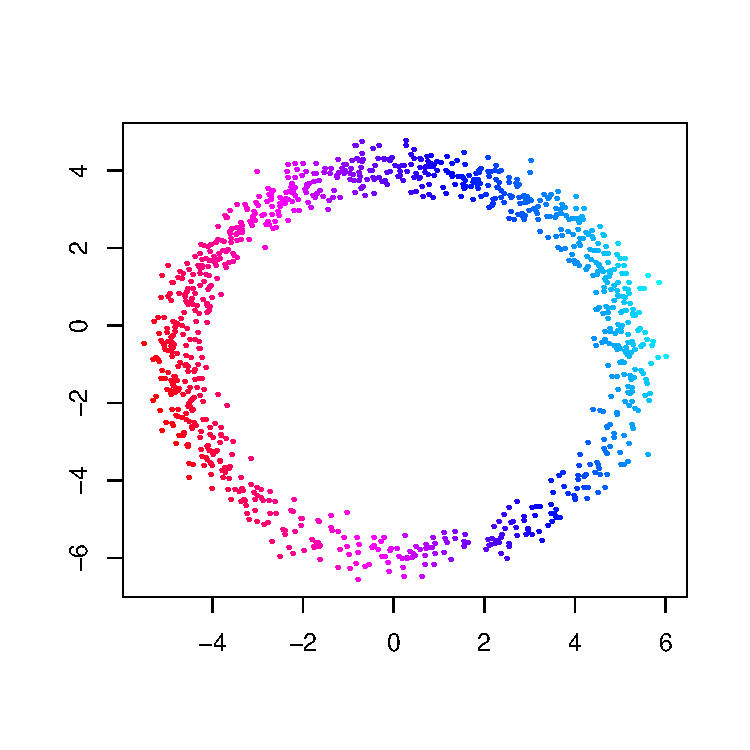
\includegraphics[scale=0.6]{mds}
	\caption{Linear MDS performed on data where linear distribution fits badly. The colors of points are defined by their projections on the components given by linear MDS.}\label{fig:mds}
\end{minipage}\hfil\begin{minipage}{0.4\columnwidth}\centering
	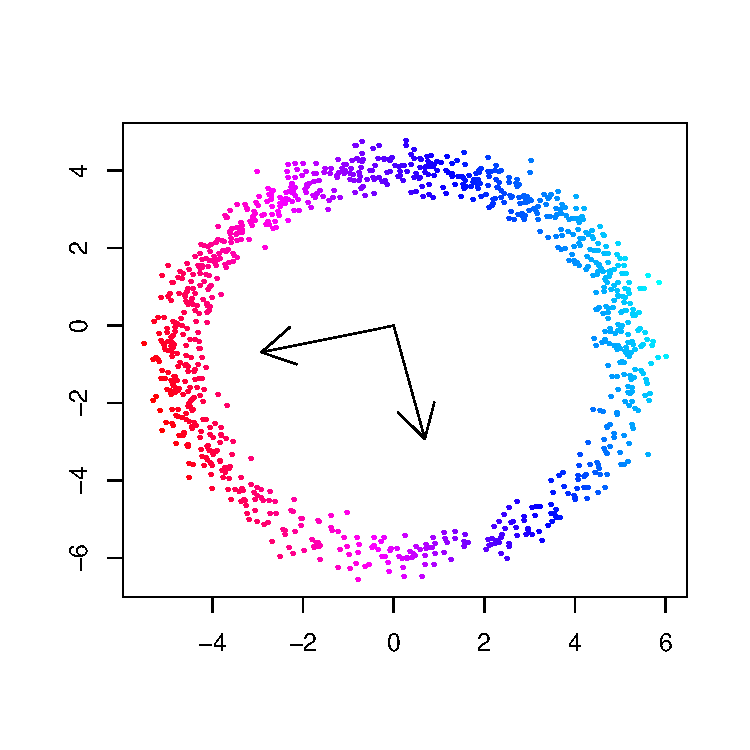
\includegraphics[scale=0.6]{mdspca}
	\caption{Result of doing PCA on the given data. The principal components are shown as arrows and the data points are colored according to their projection to the first principal components. The projections are equal to those given by linear MDS.}\label{fig:mdspca}
\end{minipage}\end{figure}

\subsection{Exercise 2}
As discussed in Section~\ref{sec:ex21}, PCA gives the same result as linear MDS, as is displayed in Figure~\ref{fig:mdspca}.

\subsection{Exercise 3}
The self-orginizing map is a way to perform nonlinear projection and clustering by finding a set of model vectors that act as cluster centers and have some predefined neighborhood relations between them.
We implemented a simple SOM algorithm where the model vectors form a chain where adjacent vectors are neighbors of each other.
The algorithm clusters the data similarly to k-means by starting at some initial configuration and iteratively assigning points to clusters and centering the model vectors according to their points in the clusters.
The difference is that instead of centering each model vector $v$ only according to the points assigned to their cluster, the points assigned to the neighbors of $v$ also affect the placement of $v$.

As with k-means, the algorithm only finds some local optimum and gives no guarantees on the quality of the solution.
Figure~\ref{fig:som} displays the result of applying the algorithm to a given data set using different numbers of model vectors.
It can be seen that in some cases the algorithm finds the "correct" nonlinear interpretation of the data, but sometimes it converges into a bad local optimum.

\begin{figure}\centering
	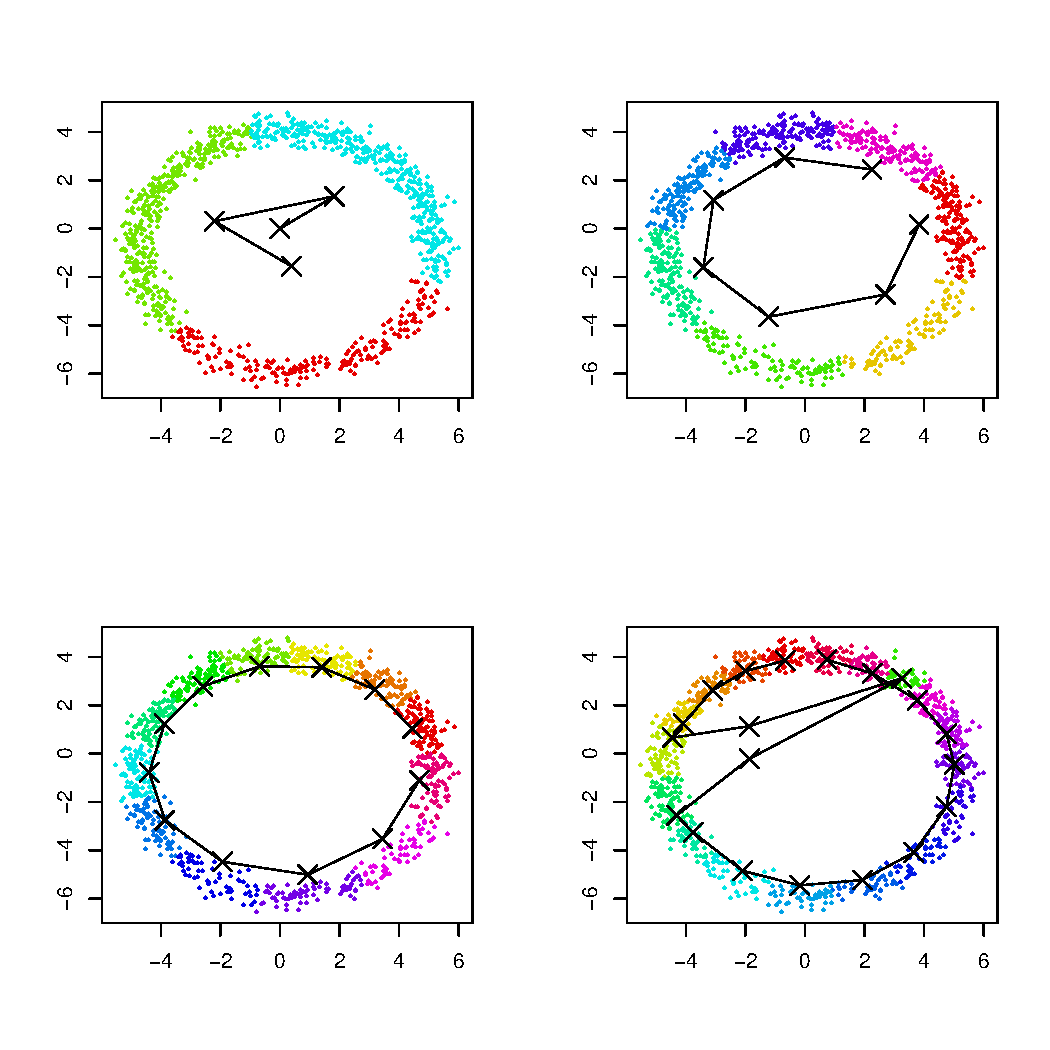
\includegraphics[width=\columnwidth]{som}
	\caption{Results of applying the SOM algorithm to data using 4, 7, 12 and 20 clusters. The algorithm may converge to a different local optimum depending on the starting point, and in the cases with 4 and 20 clusters the result is clearly suboptimal.}\label{fig:som}
\end{figure}

\subsection{Exercise 4}
We splitted each of the provided images into pacthes of size $10\times10$ pixels and composed those patches into a single matrix of size $100\times 15696$.
Each patch is considered to be a realization of a random 100-dimensional vector \vec v.
Since the patches come from different images, the distribution of \vec v is a mixture of the distributions defined by each of the images.
This differs from the distribution of the image data in the project~2, exercise~3: there each sample was a linear combination of several random variables, here each sample comes from a single distribution but the source distribution is chosen randomly.
Another difference is that in the earlier exercise each pixel was assumed independent, whereas here the variables are $10\times 10$ pixel patches and we don't assume independence between pixels of the same patch.

\subsection{Exercise 5}
We preprocessed the patches by centering each of them around zero and scaled them to unit variance.
After that we applied the SOM algorithm to the preprocessed patches, receiving a sequence of $10\times 10$ pixel images as output.
The results using 10, 20 and 30 model vectors are shown in Figure~\ref{fig:patch}.
The patches are so small that it is impossible to recognize any features of the original images from the resulting model vectors.
Instead it can be seen that model vector represents some region of the patch and adjacent model vectors represent almost the same region.

\begin{figure}
	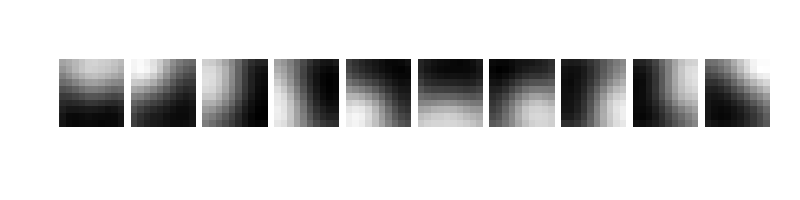
\includegraphics[width=\columnwidth]{patch10}
	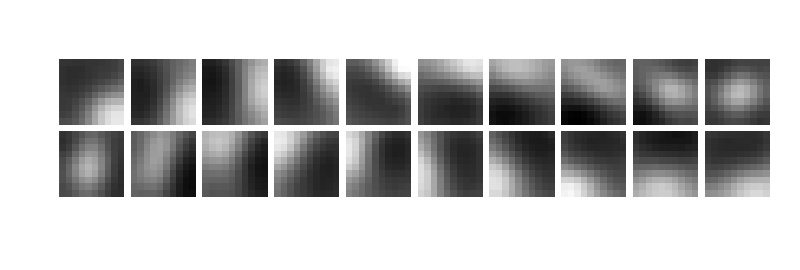
\includegraphics[width=\columnwidth]{patch20}
	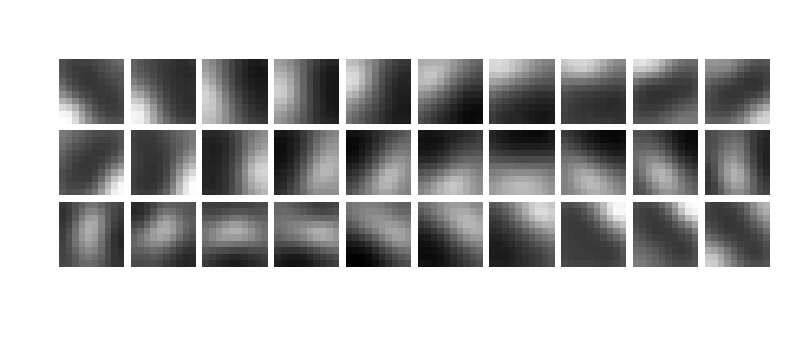
\includegraphics[width=\columnwidth]{patch30}
	\caption{SOM algorithm applied to image patches with 10, 20 and 30 model vectors. The neighbor relations between the model vectors make adjacent vector images look similar.}\label{fig:patch}
\end{figure}

\end{document}
